\documentclass[12pt]{article}

\usepackage{graphicx}

\title{E-Vote}
\author{}

\begin{document}
\maketitle

\section{Introduction}

In this paper we descrived E-Vote a simple platform for online voting. Many online groups occasionally have the necessity of voting to elect a president, new members, or make collective decisions. These groups tend to have similar characteristics: members of the group communicate primarily via email (maling lists), members do not personally know each other and may not trust other members or managers of the group, members have various level of interest and engagement in the decisions of the community and are easily turned off by complex voting procedures.

We developed the E-Vote system to provide a service to these communities. The system has the following characteristics:
\begin{itemize}
\item The system is open source and anybody can check the source code. The code is small and written in the Python language. This makes it easy for professionals in the field to check it.
\item The system can run as a service and one installation can run mutiple elections. Anybody can login into the system, create a new election, register voters and managers, and customize the ballot using an easy to use WYSIWYG interface.
\item The system communicates with voters and managers by email.
\item Voters do not need to login into the system to vote. They only need to click on the link in the notification email, fill a web form and submit.
\item Each voter can only vote once per election.
\item Results are computed automatically at closing of the election and published.
\item Voting is completely anonymous. Even a hacker with a complete database dump of the system would not be able to link voters to ballots.
\item Each voter can check at any time that his vote has been properly recorded and not alatered.
\item Each voter can independenty and at any time perform an election recount.
\item Upon voting, each voter receives an email recipt containing a copy of their filled and anonymized ballot.
\item Managers are notified by email when a new vote is cast and receive a copy of the anonimized ballot. 
\item All ballots, anonymized and digitally signed, are published, along with instruciton to verify the digital signature.
\end{itemize}

\section{Workflow}

When a new user of the system wishes to create and run a new election, the user needs to login (voting does not require login, only managing an election requires login). We will refer to this user as the election officer.
\begin{center}
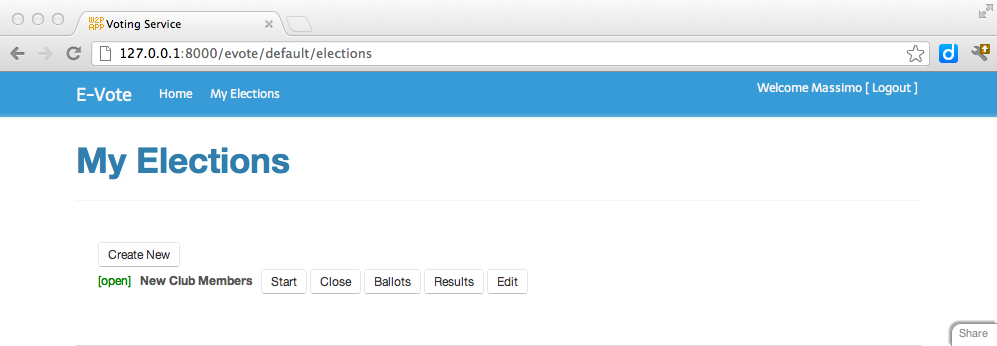
\includegraphics[width=3in]{images/elections.png}
\end{center}
The election officer can create a new election by clicking on a button, editing the content of the model ballot, listing the emails of voters and those of the election managers, and declaring the election deadline. Election managers are users to be notified when a new vote is cast. The officer is also a manager.
\begin{center}
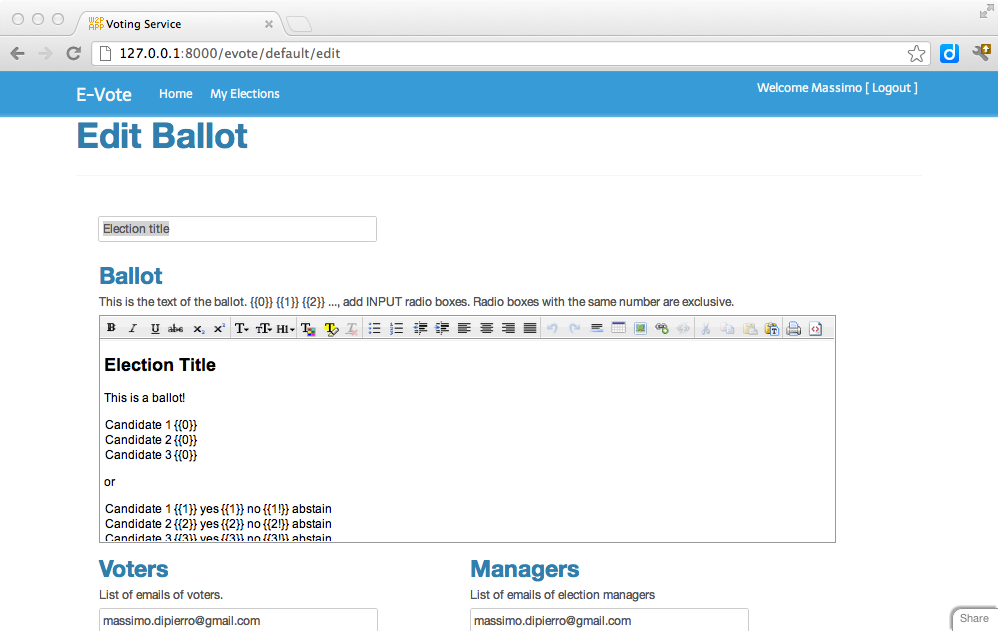
\includegraphics[width=4in]{images/edit.png}
\end{center}
The model ballot is created using a WYSIWYG syntax similar to MS Word but using only the browsers. Special tags like \{\{0\}\} allow to insert radio boxes into the ballot. The voters will check these radio boxes. Two or more radio boxes identified by the same code belong to the same radio group and are exclusive. For example:
\begin{verbatim}
Do you agree? {{0}} yes or {{0}} no
\end{verbatim}
Groups of radio boxes identified by different code are independent. For example:
\begin{verbatim}
Do you agree with A? {{0}} yes or {{0}} no
Do you agree with B? {{1}} yes or {{1}} no
\end{verbatim}
After the election is created, it can be tested, and edited. New voters and managers can be added. Voters and managers do not have to be previous users of the system and do not need an account. The election starts by emailing memebrs:
\begin{center}
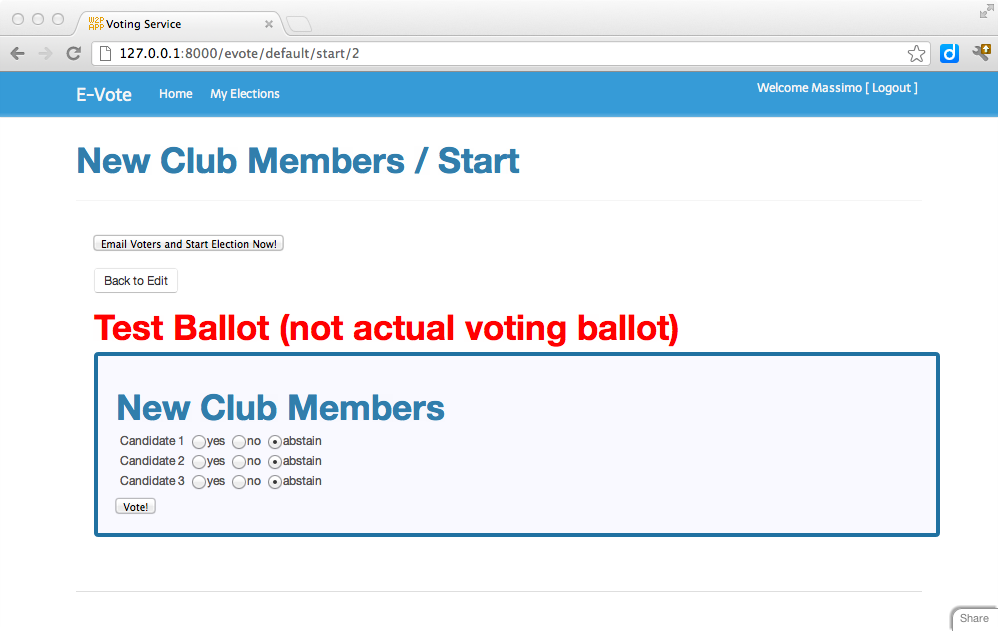
\includegraphics[width=4in]{images/start.png}
\end{center}
Each email listed by the officer corresponds to a voter. When the election starts a new record is created in the system for each voter. A voter record is uniquely identified by a {\tt voter-uuid} code. UUID stands for a Universal Unique IDentifier. It is a long random sequence of characters that is impossible to guess. The {\tt voter-uuid} is used to build a unique, one-time link, which is email to the voter and allow the user to vote.
\begin{center}
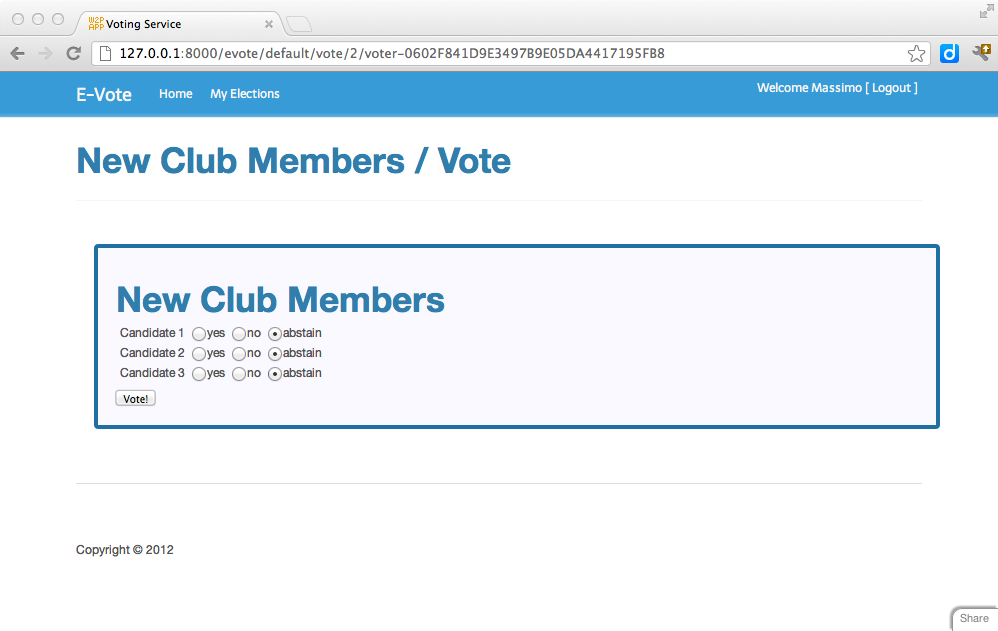
\includegraphics[width=4in]{images/vote.png}
\end{center}
The system recognizes the user from the {\tt voter-uuid} in the URL.

When the election starts, the system also generates one ballot for each voter. A ballot is a BLANK form with a unique ID for the form {\tt ballot-in} where {\tt id} is comprised on an election id and a ballot id. Ballots are not linked to the voters at this time.

When a user fills and submits the voting form, the system picks a random ballot and records the vote on that ballot. The filled ballot, containing the vote and a unique {\tt ballot-id}. The ballot is the digitally signed using the RSA algorithm using a private key associated to the election and only known to the system. The completed ballot, anonymized and signed, is published online, emailed to the user as a receipt, and emailed to the managers.

\begin{center}
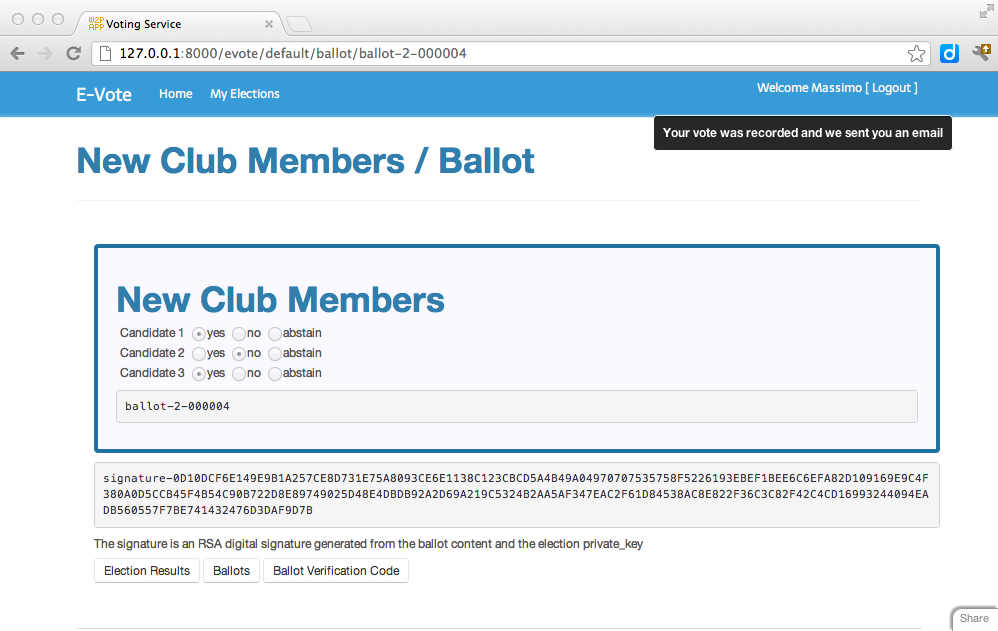
\includegraphics[width=4in]{images/ballot.png}
\end{center}
At this point the system has recorded that this voter has voted and its {\tt voter-uuid} will no longer be useful for voting. The voter can check his vote was recorded because he received a receipt with a copy of the completed ballot.

When the election starts, the system also published a complete list of {\tt ballot-id}. This allows everybody to check that new ballots have not been forged and some existing ballots have been used for voting.

\begin{center}
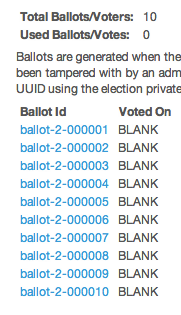
\includegraphics[width=2in]{images/ballots.png}
\end{center}

When the election is closed, results become public. The election is completely recounted evey time the {\tt results} page is visited. The system counts how many times each checkbox has been clicked.

\begin{center}
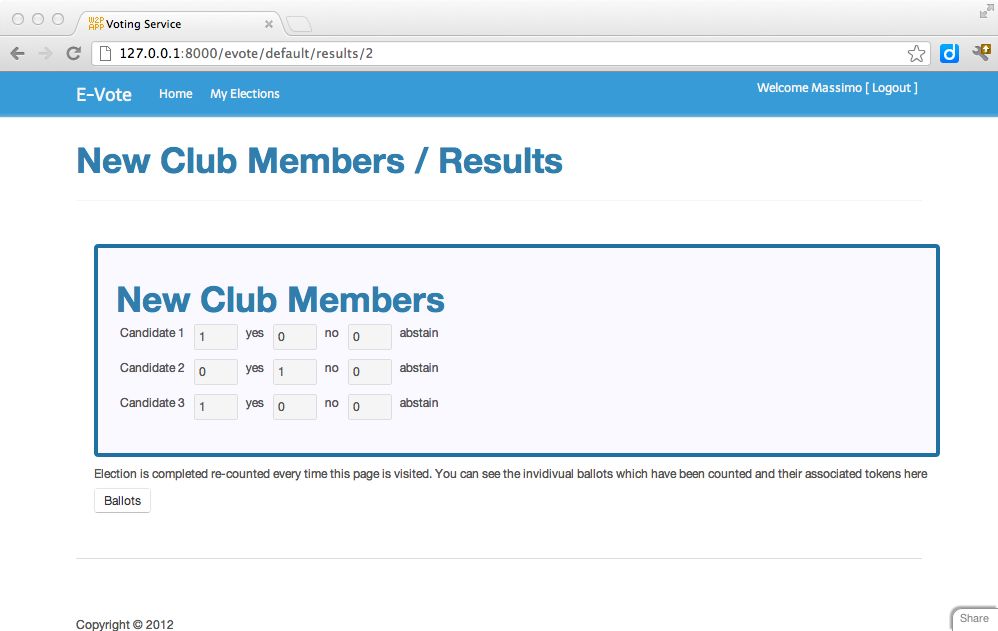
\includegraphics[width=4in]{images/results.png}
\end{center}

When the election closes some users may not have voted. They still need prof that their ballot is empty and has not been used by somebody else. For this purpose at closing of the election, the system emails every user who has not voted one of the remaining blank ballot as receipt.

\begin{center}
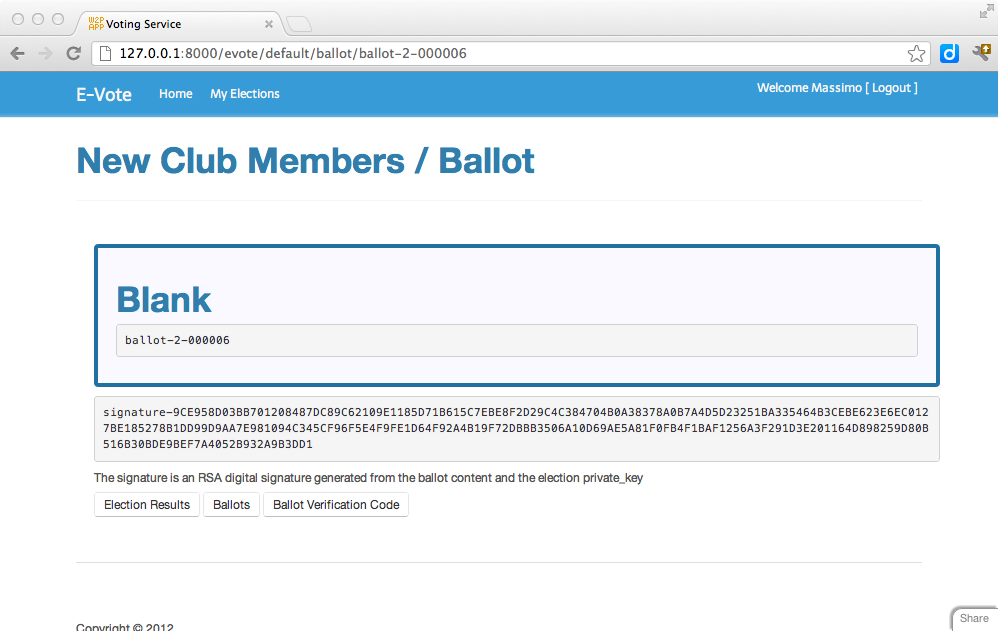
\includegraphics[width=4in]{images/ballot-blank.png}
\end{center}

In this way every user receive a receipt with a copy of their ballot (blank or filled).


\begin{verbatim}
https://127.0.0.1:8000/evote/default/elections
https://127.0.0.1:8000/evote/default/start/2
https://127.0.0.1:8000/evote/default/close_election/2
https://127.0.0.1:8000/evote/default/ballots/2
https://127.0.0.1:8000/evote/default/results/2
https://127.0.0.1:8000/evote/default/edit/2
https://127.0.0.1:8000/evote/default/vote/2/voter-160D...BE91
https://127.0.0.1:8000/evote/default/ballot/ballot-2-1
\end{verbatim}

\begin{verbatim}
ballot-2-1
\end{verbatim}

\begin{verbatim}
signature-5CF7...E246
\end{verbatim}

\begin{verbatim}
-----BEGIN RSA PUBLIC KEY-----
MIGJAoGBAMTZTDA2xdl1DFisptWMVFdEt3gj+ROKrP3lYbntvJnPBzqf1/gmTqKb
rqzmQ+uSv6P5FIR1nuFX+17LBDjg0Ovz5bFYHxWYdRy4ObktUlvH+wOs0Byi7k0z
8ZAKIKJYJQgpZptS0rqxXRqREHmEyPKT5aE6oiL9AAEvKoVxuVmrAgMBAAE=
-----END RSA PUBLIC KEY-----
\end{verbatim}

\section{Validation Process}

\begin{verbatim}
# import required libraries
import base64, rsa # install module with "pip install rsa".

# this is the ballot to verify
ballot = """
<div class="ballot"><h2>Election Title</h2>

<p>This is a ballot!</p>

<table>
<tbody><tr><td>Candidate 1</td><td><input disabled="disabled" name="ck_0" type="radio" value="1" /></td></tr>
<tr><td>Candidate 2</td><td><input checked="checked" disabled="disabled" name="ck_0" type="radio" value="2" /></td></tr>
<tr><td>Candidate 3</td><td><input disabled="disabled" name="ck_0" type="radio" value="3" /></td></tr>
</tbody></table>

<p>or</p>

<table>
<tbody><tr><td>Candidate 1</td><td><input checked="checked" disabled="disabled" name="ck_1" type="radio" value="1" /> yes</td><td><input disabled="disabled" name="ck_1" type="radio" value="2" /> no</td><td><input disabled="disabled" name="ck_1" type="radio" value="3" /> abstain</td></tr>
<tr><td>Candidate 2</td><td><input checked="checked" disabled="disabled" name="ck_2" type="radio" value="1" /> yes</td><td><input disabled="disabled" name="ck_2" type="radio" value="2" /> no</td><td><input disabled="disabled" name="ck_2" type="radio" value="3" /> abstain</td></tr>
<tr><td>Candidate 3</td><td><input checked="checked" disabled="disabled" name="ck_3" type="radio" value="1" /> yes</td><td><input disabled="disabled" name="ck_3" type="radio" value="2" /> no</td><td><input disabled="disabled" name="ck_3" type="radio" value="3" /> abstain</td></tr>
</tbody></table><pre>
ballot-2-1
</pre></div>
""".strip()

# this is the ballot RSA signature
signature = base64.b16decode("5CF72361F326D5980C8B031DA8D7B4279AE29E592DD49633C73232F7CD752D05DE32C09A359D44AB2D243FBBAA2185872CC3CB0A26EFDBAFDB69B207FD97B4D13B87E8421B848C817D191A97A3B5BB377637975AA4C52C81DF35E2B29B8B9F9D9B0E6E0473071E1D2279BC5A7434DB620AD4D7A7E22DBB711782CF614EAEE246")

# this is the election public key
pk_pem = """
-----BEGIN RSA PUBLIC KEY-----
MIGJAoGBAMTZTDA2xdl1DFisptWMVFdEt3gj+ROKrP3lYbntvJnPBzqf1/gmTqKb
rqzmQ+uSv6P5FIR1nuFX+17LBDjg0Ovz5bFYHxWYdRy4ObktUlvH+wOs0Byi7k0z
8ZAKIKJYJQgpZptS0rqxXRqREHmEyPKT5aE6oiL9AAEvKoVxuVmrAgMBAAE=
-----END RSA PUBLIC KEY-----
"""

# this is the code that verifies the signature
public_key = rsa.PublicKey.load_pkcs1(pk_pem)
if rsa.verify(ballot, signature, public_key)==None:
    print 'valid'
else:
    print 'invalid'
\end{verbatim}

\section{Conclusions}

\begin{thebibliography}{999}
\bibitem{test} ...
\end{thebibliography}
\end{document}
